\documentclass[../thesis.tex]{subfiles}

\begin{document}

\chapter{Anwendung}

In diesem Kapitel werden die Ergebnisse des Benchmarks, welcher mit der in \texttt{TREND} vorhandenen Zustandsgleichung \texttt{PSRK} durchgeführt wurde gezeigt. Anschließend werden die Ergebnisse mit Literaturdaten verglichen und Gründe für die resultierenden Abweichungen genannt.

\section{Berechnungsergebnisse}

Die Anwendung des Benchmarks mit dem Modell der \texttt{PSRK} führt zu den in \autoref{tab: meine_bac_ergebnisse} dargestellten Gruppenergebnissen.

\begin{table} [htb]
	\centering
	\caption{\texttt{TREND} Berechnungsergebnisse pro Gruppe mit dem Modell \texttt{PSRK}}
	\begin{tabular}{ cccccccc }
		\hline
		BAC & $ x $ & $ y $ & $ p_\mathrm{az}$ & $ x_\mathrm{az}$ & $ h^\mathrm{M} $ & $ c_p^\mathrm{M} $ & \textbf{Gesamtnote} \\
		\hline
		1 & 11.18 & 10.88 & -     & -     & 10.62 & 8.88  & \textbf{10.39}\\
		2 & 8.63  & 10.39 & 16.77 & 12.68 & 9.42  & 9.54  & \textbf{11.24}\\
		3 & 9.90  & 10.72 & 5.34  & 18.54 & 5.90  & 12.03 & \textbf{10.40}\\
		4 & 10.51 & 13.80 & 0.0   & 0.0   & 4.62  & 12.0  & \textbf{6.82}\\
		5 & 10.74 & 8.29  & 0.0   & 0.0   & 6.72  & 13.03 & \textbf{6.46}\\
		6 & 8.88  & 7.10  & 0.0   & 2.37  & 5.47  & 6.61  & \textbf{5.07}\\
		7 & 9.60  & 11.47 & 9.76  & 6.73  & 1.40  & 0.0   & \textbf{6.49}\\
		8 & 7.53  & 9.77  & 8.06  & 8.65  & 5.24  & 8.47  & \textbf{8.65}\\
		9 & 9.75  & 10.81 & 9.29  & 8.38  & 6.73  & 3.04  & \textbf{8.00}\\
		\hline
		\label{tab: meine_bac_ergebnisse}
	\end{tabular}
\end{table}


Aus den Gruppenergebnissen ergeben sich die in \autoref{tab: meine_gesamt_ergebnisse} aufgeführten Klassenergebnisse.

\begin{table} [htb]
	\centering
	\caption{\texttt{TREND} Berechnungsergebnisse pro Klasse mit dem Modell \texttt{PSRK}}
	\begin{tabular}{ ccc }
		\hline
		Gruppe & BACs & Note  \\
		\hline
		NA & 1-4 & 9.71 \\
		SA & 5   & 6.46 \\
		CA & 6   & 5.07 \\
		CA+SA & 7-9 & 7.48 \\ 
	
		\hline
		\label{tab: meine_gesamt_ergebnisse}
	\end{tabular}
\end{table}

Die Gesamtnote des Modells kann nach \autoref{eq: mark_final} aus den Klassenergebnissen berechnet werden und hat in diesem Fall einen Wert von \textbf{7.18}.

\section{Literaturvergleich}

In \cite{bibid} wurde der beschriebene Benchmark ebenfalls mit der \texttt{PSRK} durchgeführt. Die dort erhaltenen Klassenergebnisse sind in \autoref{tab: PSRK benchmark literatur bac} und die Gruppenergebnisse in \autoref{tab: PSRK benchmark literatur gruppen} aufgeführt.

\begin{table} [htb]
	\centering
	\caption{Literatur Berechnungsergebnisse pro Gruppe mit dem Modell \texttt{PSRK}}
	\begin{tabular}{ cccccccccccc }
		\hline
		BAC & $ x $ & $ y $ & $ p_\mathrm{c}$ & $ x_\mathrm{c}$ & $ p_\mathrm{az}$ & $ x_\mathrm{az}$ & $ p_\mathrm{LLV}$ & $ z_\mathrm{LLV}$ & $ h^\mathrm{M} $ & $ c_p^\mathrm{M} $ & \textbf{Gesamtnote} \\
		\hline
		1 & 12.9 & 16.3 & 16.0  & 11.6  & 19.2  & 18.6 & 18.1 & 7.9  & 6.0  & 0.3 & \textbf{12.7}\\
		2 & 14.3 & 15.6 & 17.3  & 14.7  & 19.1  & 16.0 & -    & -    & 11.6 & 3.4 & \textbf{14.0}\\
		3 & 0.0  & 7.7  & 16.0  & 3.1   & 13.3  & 7.5  & -    & -    & 3.7  & 0.0 & \textbf{6.4}\\
		4 & 10.8 & 12.7 & 16.8  & 12.1  & 17.8  & 13.3 & -    & -    & 7.0  & 0.0 & \textbf{11.3}\\
		5 & 10.3 & 14.8 & 11.1  & 0.0   & 19.1  & 17.3 & 18.5 & 0.0  & 10.6 & 7.7 & \textbf{10.9}\\
		6 & 0.4  & 9.9  & 16.9  & 15.4  & 15.2  & 8.1  & -    & -    & 2.8  & 4.8 & \textbf{9.2}\\
		7 & 12.0 & 14.7 & -     & -     & 19.1  & 13.6 & -    & -    & 3.6  & 0.1 & \textbf{10.5}\\
		8 & 7.7  & 13.8 & 5.7   & 6.3   & 18.3  & 11.2 & 20.0 & 12.3 & 8.1  & 5.9 & \textbf{10.9}\\
		9 & 10.8 & 13.1 & 14.1  & 9.7   & 17.7  & 7.1  & 18.7 & 0.0  & 5.0  & 5.5 & \textbf{10.2}\\
		\hline
		\label{tab: PSRK benchmark literatur bac}
	\end{tabular}
\end{table}

Aus den Gruppenergebnissen ergeben sich die in \autoref{tab: meine_gesamt_ergebnisse} aufgeführten Klassenergebnisse.

\begin{table} [htb]
	\centering
	\caption{\texttt{TREND} Berechnungsergebnisse pro Klasse mit dem Modell \texttt{PSRK}}
	\begin{tabular}{ ccc }
		\hline
		Gruppe & BACs & Note  \\
		\hline
		NA & 1-4 & 11.1 \\
		SA & 5   & 10.9 \\
		CA & 6   & 9.2 \\
		CA+SA & 7-9 & 10.5 \\ 
		\hline
		\label{tab: PSRK benchmark literatur gruppen}
	\end{tabular}
\end{table}

Die Gesamtnote des in \cite{bibid} durchgeführten Benchmarks beträgt \textbf{10.4}.

Beim Vergleich der Ergebnisse fällt auf, dass sich deutliche Unterschiede zeigen. Um die beiden Benchmarks miteinander vergleichen zu können, werden die berechneten Systeme im Idealfall inklusive deren berechnete Daten benötigt. Aus den in \cite{bibid} vorgestellten Ergebnisse geht leider nicht hervor welche Systeme berechnet wurden. Auch ein Anteil oder die Anzahl der Systeme pro Gruppe wäre zum einordnen der Ergebnisse hilfreich. Unter den genannten Rahmenbedingung zeigt der Vergleich der Ergebnisse, dass der Benchmark korrekt implementiert wurde, da beide Ergebnisse eine plausible Größenordnung zeigen. Unabhängig davon sind weitere Tests notwendig um in \autoref{chap: fehler} noch nicht genannte Fehler aufzudecken und zu beheben.


\chapter{Fehlerquellen und Entwicklungspotential}
\label{chap: fehler}

In der bisherigen Implementation treten unter einigen Umständen Fehler bei der Bewertung einzelner Systeme auf. Dies betrifft insbesondere Größen, welche auf dem Phasengleichgewicht basieren. Dies sind damit die Größen des Phasengleichgewichts selbst $x$ und $y$, sowie die Größe des azeotropen Punkts $ x_\mathrm{az} $, da diese aus den Phasengleichgewichtsdaten bestimmt wird. Der konkrete Fehler welcher auftritt ist, dass die Lage des Phasengleichgewichts falsch eingeschätzt wird und somit die Molenbrüche der experimentellen und die der berechneten Daten nicht zueinander passen. Ein System bei dem dieser Fehler auftritt ist in \autoref{fig: phasenggw fehler1} zu sehen.

\begin{figure}[htb]
	\centering
	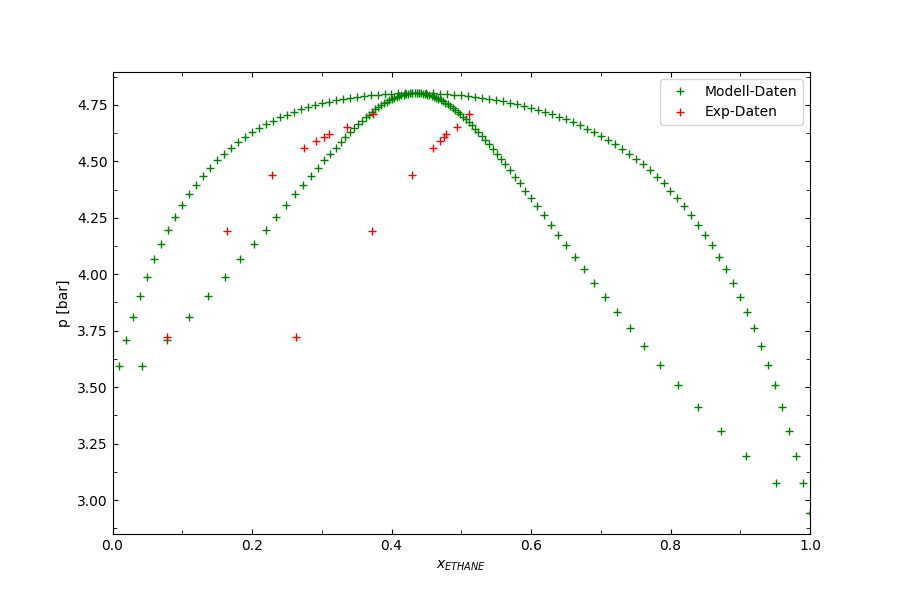
\includegraphics[scale=0.6]{CARBON DIOXIDE_ETHANE_isotherm_207_}
	\caption{Isothermes Phasengleichgewicht bei $ 207 K$ für das Stoffgemisch Kohlenstoffdioxid|Ethan}
	\label{fig: phasenggw fehler1}
\end{figure}

Die Hauptursache für diesen Fehler ist, dass die Lage der experimentellen Messdaten falsch bestimmt wird. Gerade wenn, wie in dem gezeigten Fall, die experimentellen Messdaten nur in einem Teilbereich vorliegen kommt es häufig zur falschen Einschätzung der Lage. Verbesserungen bei der Lageerkennung haben direkten Einfluss auf den berechneten Molenbruch des azeotropen Punkts sowie die Bewertung der Phasengleichgewichtsdaten.

Ein weiterer Fehler der auftritt ist, dass bei der Berechnung von isothermen Phasengleichgewichtsdaten falsche Werte für den Druck erhalten werden. Der Druck bleibt über den gesamten Wertebereich konstant, wie in \autoref{fig: phasenggw fehler2} zu sehen.

\begin{figure}[htb]
	\centering
	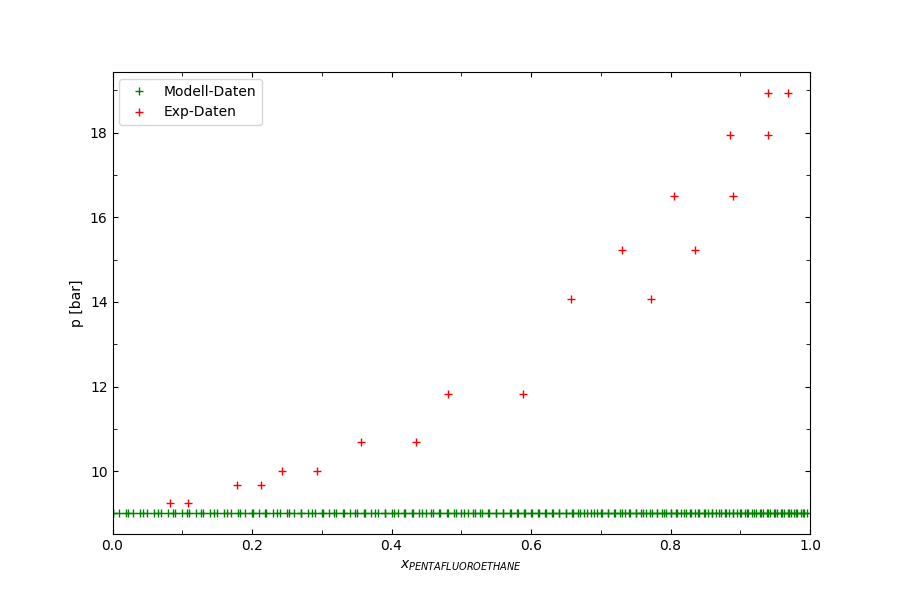
\includegraphics[scale=0.6]{PENTAFLUOROETHANE_DIMETHYL ETHER_isotherm_313.15_}
	\caption{Isothermes Phasengleichgewicht bei $ 315$.$15 K$ für das Stoffgemisch Pentaflourethan|Dimethylether}
	\label{fig: phasenggw fehler2}
\end{figure}
Der Grund für das Auftreten dieses Fehler liegt in \texttt{TREND} da bei sonstigen Fehlern ein Fehlercode generiert wird und die Berechnung fehlschlägt. 

Weitere Mögliche Ursachen für abweichende Noten können die für das Modell verwendeten Parameter sein. Alle in dieser Arbeit verwendeten Parameter sind im Ordner \texttt{TREND 4.0} an ihrer entsprechen Stelle zu finden und liegen dem Quellcode bei.


\end{document}
